\begin{figure}[htp] % (here, top of the page, the next page)
\graphicspath{{chapters/chapter4/images/alternated_move_and_push/}}
%\centering

\begin{subfigure}[t]{0.30\textwidth}
  \centering
  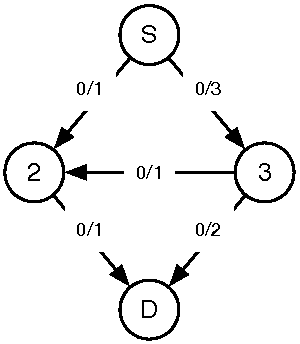
\includegraphics[width=\linewidth,height=\linewidth, keepaspectratio]{alternated_move_and_push1.pdf}
  \caption{A capacitated graph with one source $S$ and one sink $D$ node.}\label{fig:alternated_move_and_push_fig1}
\end{subfigure}
\quad
\begin{subfigure}[t]{0.30\textwidth}
  \centering
  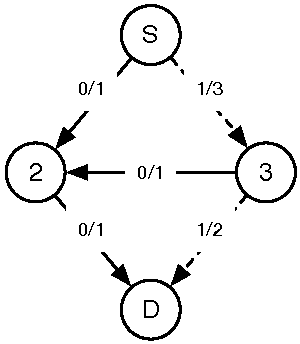
\includegraphics[width=\linewidth,height=\linewidth, keepaspectratio]{alternated_move_and_push2.pdf}
  \caption{The first trail created by an ant. The path is randomly created based on pheromone levels. A single flow unit is pushed along the the edges included in the trail. The trail is denoted by a dashed line.}\label{fig:alternated_move_and_push_fig2}
\end{subfigure}
\quad
\begin{subfigure}[t]{0.30\textwidth}
  \centering
  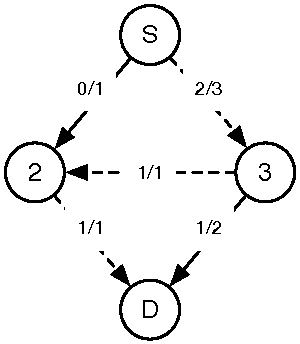
\includegraphics[width=\linewidth,height=\linewidth, keepaspectratio]{alternated_move_and_push3.pdf}
  \caption{A second pass is conducted by the same ant. This resulted in a new random path. A single flow unit is pushed along the trail.}\label{fig:alternated_move_and_push_fig3}
\end{subfigure}

\begin{subfigure}[t]{0.30\textwidth}
  \centering
  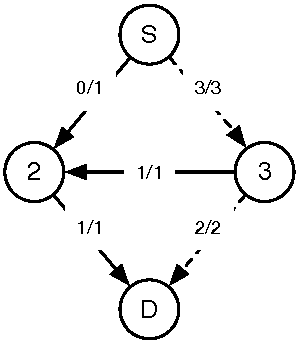
\includegraphics[width=\linewidth,height=\linewidth, keepaspectratio]{alternated_move_and_push4.pdf}
  \caption{A third pass is performed by the same ant, and a flow unit is pushed through the graph along the path.}\label{fig:alternated_move_and_push_fig4}
\end{subfigure}
\quad
\begin{subfigure}[t]{0.30\textwidth}
  \centering
  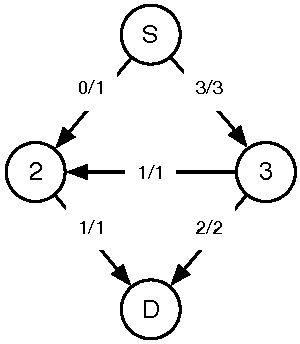
\includegraphics[width=\linewidth,height=\linewidth, keepaspectratio]{alternated_move_and_push5.pdf}
  \caption{The ant can no longer reach the sink node, and the ant therefore terminates its search for paths through the graph. The solution construction has terminated.}\label{fig:alternated_move_and_push_fig5}
\end{subfigure}


\caption{How a solution is constructed using the Alternated Move and Push strategy.}\label{fig:alternated_move_and_push_construction}
\end{figure}